\section{Hastighedsmåler}


\subsection{Komponenter}
\subsubsection{IR afsender diode - L-34F3BT}
% afsender diode

Relevante størrelser på dioden \cite{kompIRafsender} er bestemt ud fra absolute maximum ratings ved en temperatur på \SI{25}{\celsius} 
Duty cyclen er
\begin{align}
	D &= \frac{1}{100} \\
\end{align}
med en puls længde på 
\begin{align}
	PW &= \SI{10}{\micro s} \\
\end{align}

Dette betyder at KingBright har vist at dioden kan med sikkerhed klare en frekvens på
\begin{align}
	f &=  \frac{D}{PW} =  \frac{\frac{1}{100}}{\SI{10}{\micro s}} = \SI{1000}{Hz}\label{eq:oensketFrekvens}\\ 
\end{align}
Hvilket vi vil forsøge at tilnærme.

Samt kan den klare en strømstyrke på 
\begin{align}
	I_{FS} &= \SI{1.2}{A} \\
\end{align}

\subsubsection{IR modtager diode - BPW 34 FA}
% Modtager Diode
Relevante størrelser for IR modtager dioden \cite{kompIRmodtager} er at den har en kort switching tid på
\begin{align}
	t &= \SI{20}{\nano s} \\
\end{align}

Den er bygget til at opfange lys med frekvensen på
\begin{align}
	 [\SI{730}{nm};\SI{1100}{nm}] \\
\end{align}
Hvilket er fint for vores formål med infrarød lys.
\subsubsection{555 timer - NE555P}
% 555 timer
Vi benyttede en 555 timer\cite{komp555} til at producere ønskede signaler med en frekvens på \SI{1000}{Hz}, som beskrevet i ligning \ref{eq:oensketFrekvens}.
 %Duty cycle
Problemet ved at benytte en normal monostabil 555 timer er at duty cycle aldrig kan komme under $50\%$ (kilde: \cite{555timer50percent}), dette betyder at vi ikke kan producerer korte signaler som ønsket, ved direkte at udvælge bestemte modstande. Derfor udnytter vi at duty cyclen kan sættes væsentligt højere op (nær 99\%) og vi kan derfra inverterer signalet. Beregninger for udvælgelse af korrekte modstande for at få en ønsket duty cycle kan findes i afsnit \ref{calc:555timerResistance}.

% -------------___PIN diagram
\begin{figure}[H]
	\centering
    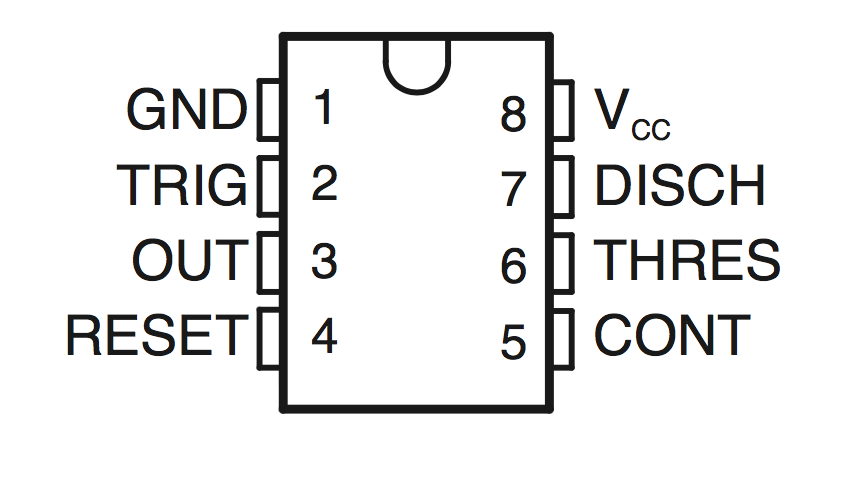
\includegraphics[height=7cm]{figures/2_4_4hastighedsmaal/komp555pin.png}
	\caption{Pindiagram over NE555P}
	\label{fig:komp555pin}
\end{figure}

\subsubsection{Signal invertering - HEF4001B}
Kilde: \cite{kompInverter}
Vi har benyttet komponenter HEF4001B som er en IC med OR gates, som vi benytter til at inverterer signalet fra 555-timeren.



% ----------- PIN DIAGRAM
\begin{figure}[H]
	\centering
    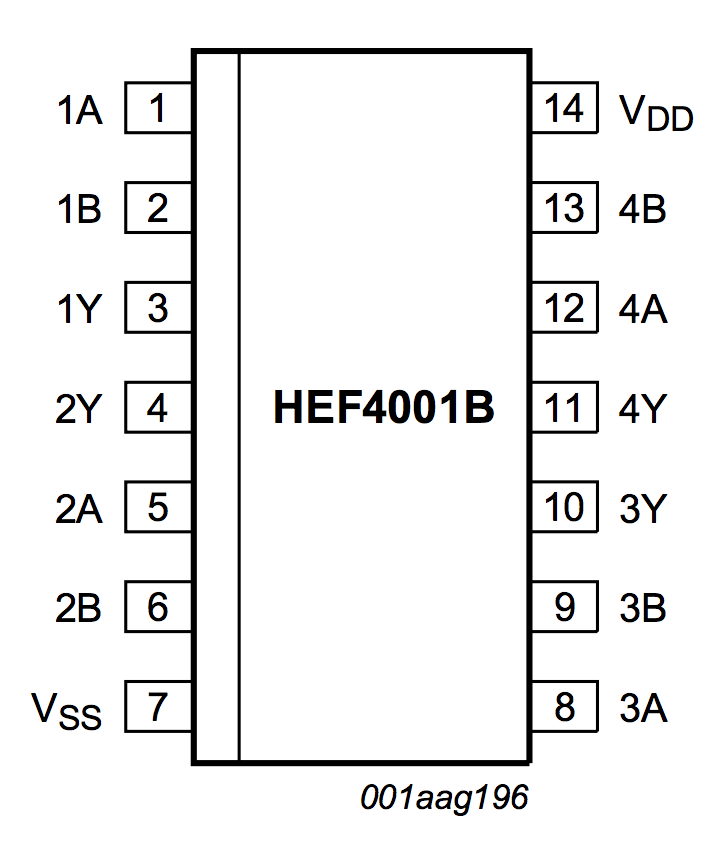
\includegraphics[height=7cm]{figures/2_4_4hastighedsmaal/kompInverterpin.png}
	\caption{Pindiagram over HEF4001B}
	\label{fig:kompInverter}
\end{figure}
% --------------


\subsection{Teori}
\subsubsection{Benyttelse af diode som variabel spænding}
\subsubsection{Nor-gate}
En norgate er en af de logiske gate der tager et digital signal som input og laver et nyt digitalt signal som output baseret på hvilke dens input. I vores tilfælde havde vi tænkt os at bruge en not gate til at invatere vores input. Men siden at det var nemmere at få fat på en nor-gate i stedet for en not gate har vi brugt den i stedet for og sat den ene inputpin til ground så den fungere ligesom en notgate.
\subsubsection{Hastighedsmålingsmetoder}
% \subsubsection{2 sensorer}
% \subsubsection{Knap og sensor}
Tidsmålingen bestemmes ved at vi kender et hvis strækning bolden har bevæget sig i, samt at man kender det tidsinterval bolden bevæger sig strækningen. Således bestemmes hastigheden:
\begin{align}
	v_{bold} &=\frac{\Delta s}{\Delta t} \\
\end{align}
 Heraf er der to løsninger til at bestemme dette.
Den ene er at benytte to infrarød afsender og modtagere kredse, som er sat sammen i par. Således at når den første del registrerer at en bold passerer undervejs så begyndes der at tage tid, indtil den næste del registrerer at bolden passerer. 

Den anden metode er at benytte en infrarød afsender og modtager-kreds og en knap, så når der trykkes på knappen tages der tid fra at bolden skydes af sted til at den registreres af infrarød afsender og modtager kreds.

Vi endte med at vælge den anden metode, grundet tidspres da vi efter vores fremstilling stødte på problemer, da kredsløbet ikke fungerede på PCB. Se afsnit \ref{subs:endeligProto}.
\todo{Hold øje med om der refereres til det rigtige afsnit}








\subsection{Beregninger}
\todo{mangler nogle enkelte beregninger}
\subsubsection{555 timer modstande} \label{calc:555timerResistance}
For 555 gælder det at vi ønsker en frekvens på 
\[
	f_{target} =  \SI{1000}{\hertz}
\]

Der kan opstilles 4 ligninger for 555 timeren således: 
For mark-time gælder det at
\begin{align}
	T_m &= 0.7 \cdot C_1 \cdot (R_1 + R_2) \label{eq:marktime} \\
\end{align}
For space-time gælder det at 
\begin{align}
	T_s &= 0.7 \cdot C_1 \cdot (R_2) \label{eq:spacetime} \\
\end{align}

For perioden gælder det at 
\begin{align}
	T &= \frac{1}{f} = T_s + T_m \label{eq:periodtime} \\
\end{align}
Og da dutycyclen skal være så tæt på $100$ som muligt sættes følgende forhold til at gælde
\begin{align}
	T_m &= 100 \cdot  T_s \label{eq:dutycycle} \\
\end{align}
Ved at løse ligningssystemet for ligningerne \ref{eq:spacetime}, \ref{eq:dutycycle}, \ref{eq:marktime}, \ref{eq:periodtime}, og isolerer for $R_1$ og $R_2$ og opskriver den som funktion af kapacitoren og frekvensen fås udtrykkende:
\begin{align}
	R_{1} \left( C_1,f \right) &= 1.400\,{\frac {1}{f \cdot C_1}} \\[2ex]
	R_{2} \left( C_1,f \right) &= 0.01414\,{\frac {1}{f \cdot C_1}}
\end{align}
Så antages at kondensatoren er 
\[
	C_1 = \SI{1.0d-6}{\farad}
\]
Da det antages vi bare benytter standardværdien. \todo{Er det standardværdien?***}

Frekvensen er nævnt og således bliver modstandende
\begin{align}
	R_1(\SI{1.0d-6}{\farad},\SI{1000}{\hertz})&= \SI{1400}{\ohm} \\[1ex]
	R_2(\SI{1.0d-6}{\farad},\SI{1000}{\hertz})&= \SI{14.14}{\ohm}
\end{align}

\subsubsection{Bestemmelse af modstande for peak-detektoren}

Vi har besluttet at benytte en peak-detektor til at opfange IR signalet til modtageren. Heraf benyttes der en simpel peak-detektor opbygning\todo{Er det den rigtige betegnelse***}.  Udtryk og teori benyttet er fra kilde \cite{peakdetectorCalc}.

Ud fra diodens karakteristika fås en forward-biased resistans på
\[
	r_{df} = \SI{607}{\ohm}
\]
og en reversed bias resistens på
\[
	r_{dr} = \SI{2d7}{\ohm}
\]
Således gælder det at vi skal vælge en modstand $R$ hvor det gælder at
\[
	r_{df} < R < r_{dr}
\]
Vores tidsvariable \todo{Rigtig betegnelse?} $\tau_2$ kan defineres som
\[
	\tau_2 = R \cdot C
\]
hvor $C$ er kapacitoren vi benytter i peakdetektoren.

\subsection{Test}
\todo{Der skal nok referes til billeder og navne på komponenter i billedet når der snakkes om tests***} 
\subsubsection{Afsender dioden}
Vi testede 555-timeren med et PC-oscilloskop.

På Figur ~\ref{fig:555noninv} er der en graf af den 555-timerens output, som det fremgår på info-boksene er duty cyclen er høj som beregnet. Det bemærkes også at frekvensen er lidt større end $\SI{1000}{Hz}$ men vi forventer ikke det giver os problemer.

Det inverterede signal kan ses på \ref{fig:555inv} og det fungerer som ønsket.
\begin{figure}[H]
	\centering
    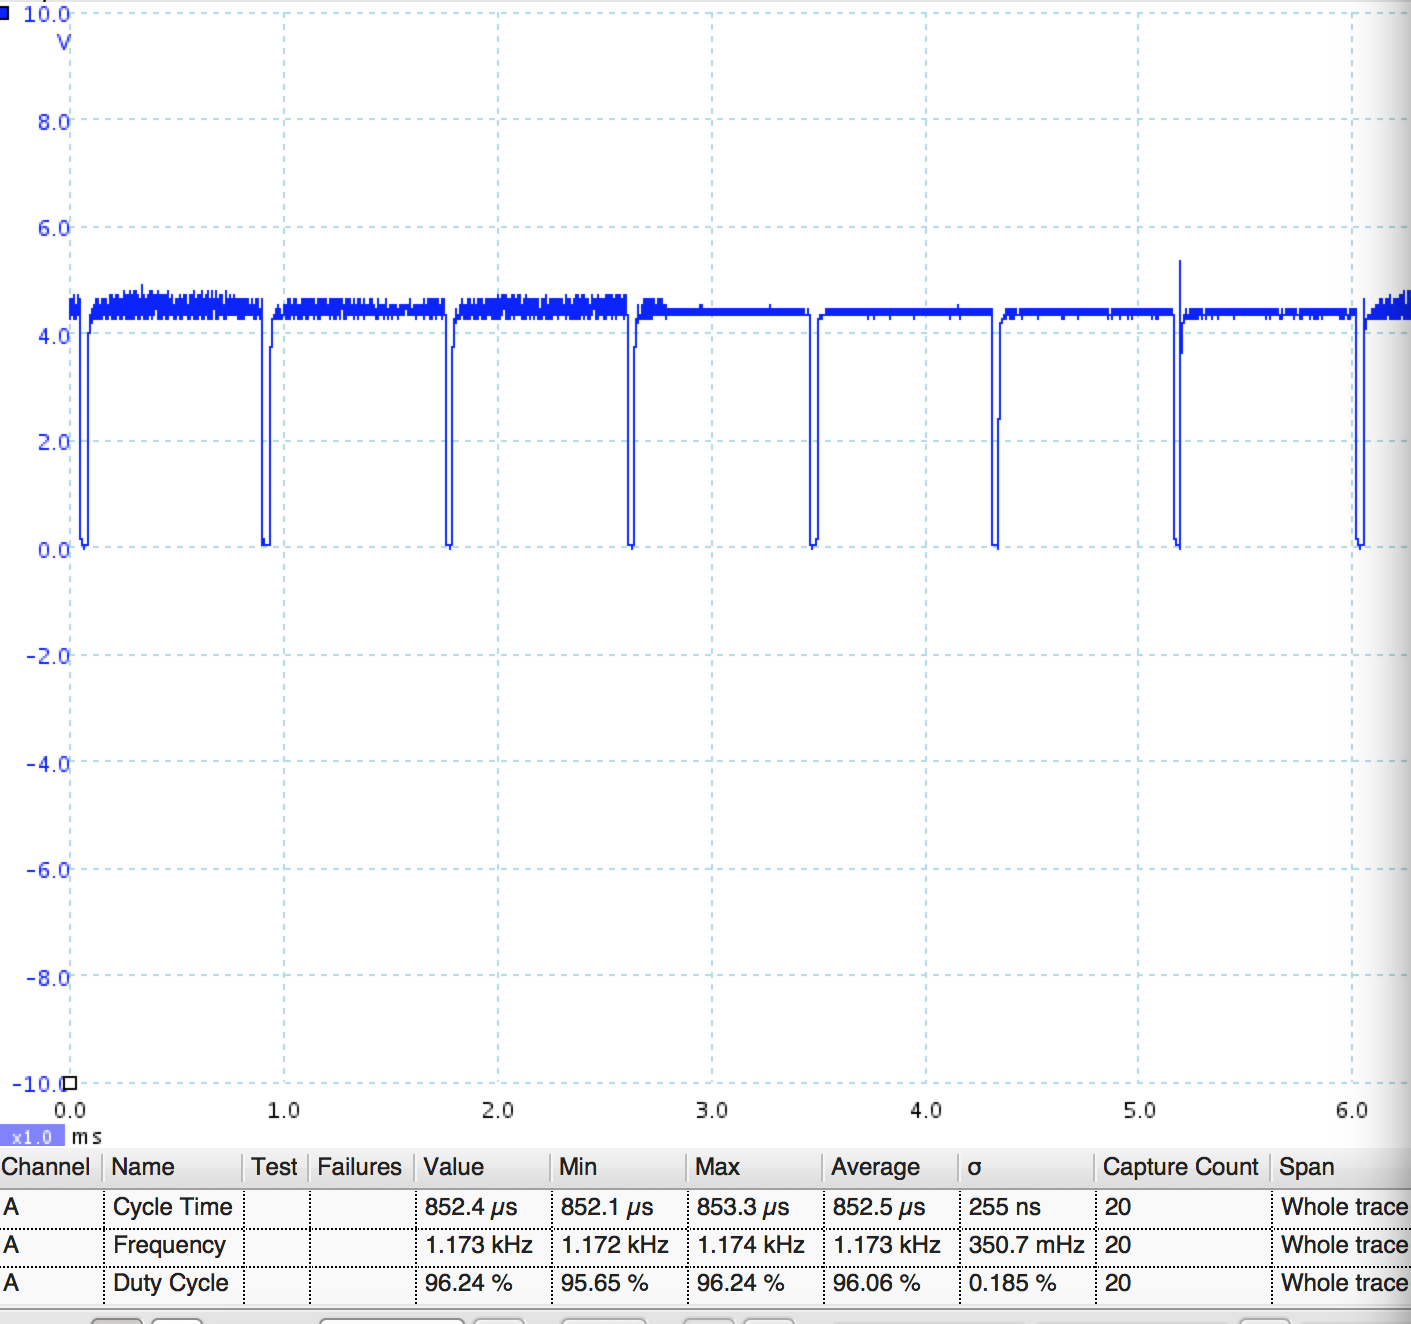
\includegraphics[width=13cm]{figures/2_4_3hastighed/555signal.png}
	\caption{Spænding som funktion af tiden med info-bokse i bunden}
	\label{fig:555noninv}
\end{figure}

\begin{figure}[H]
	\centering
    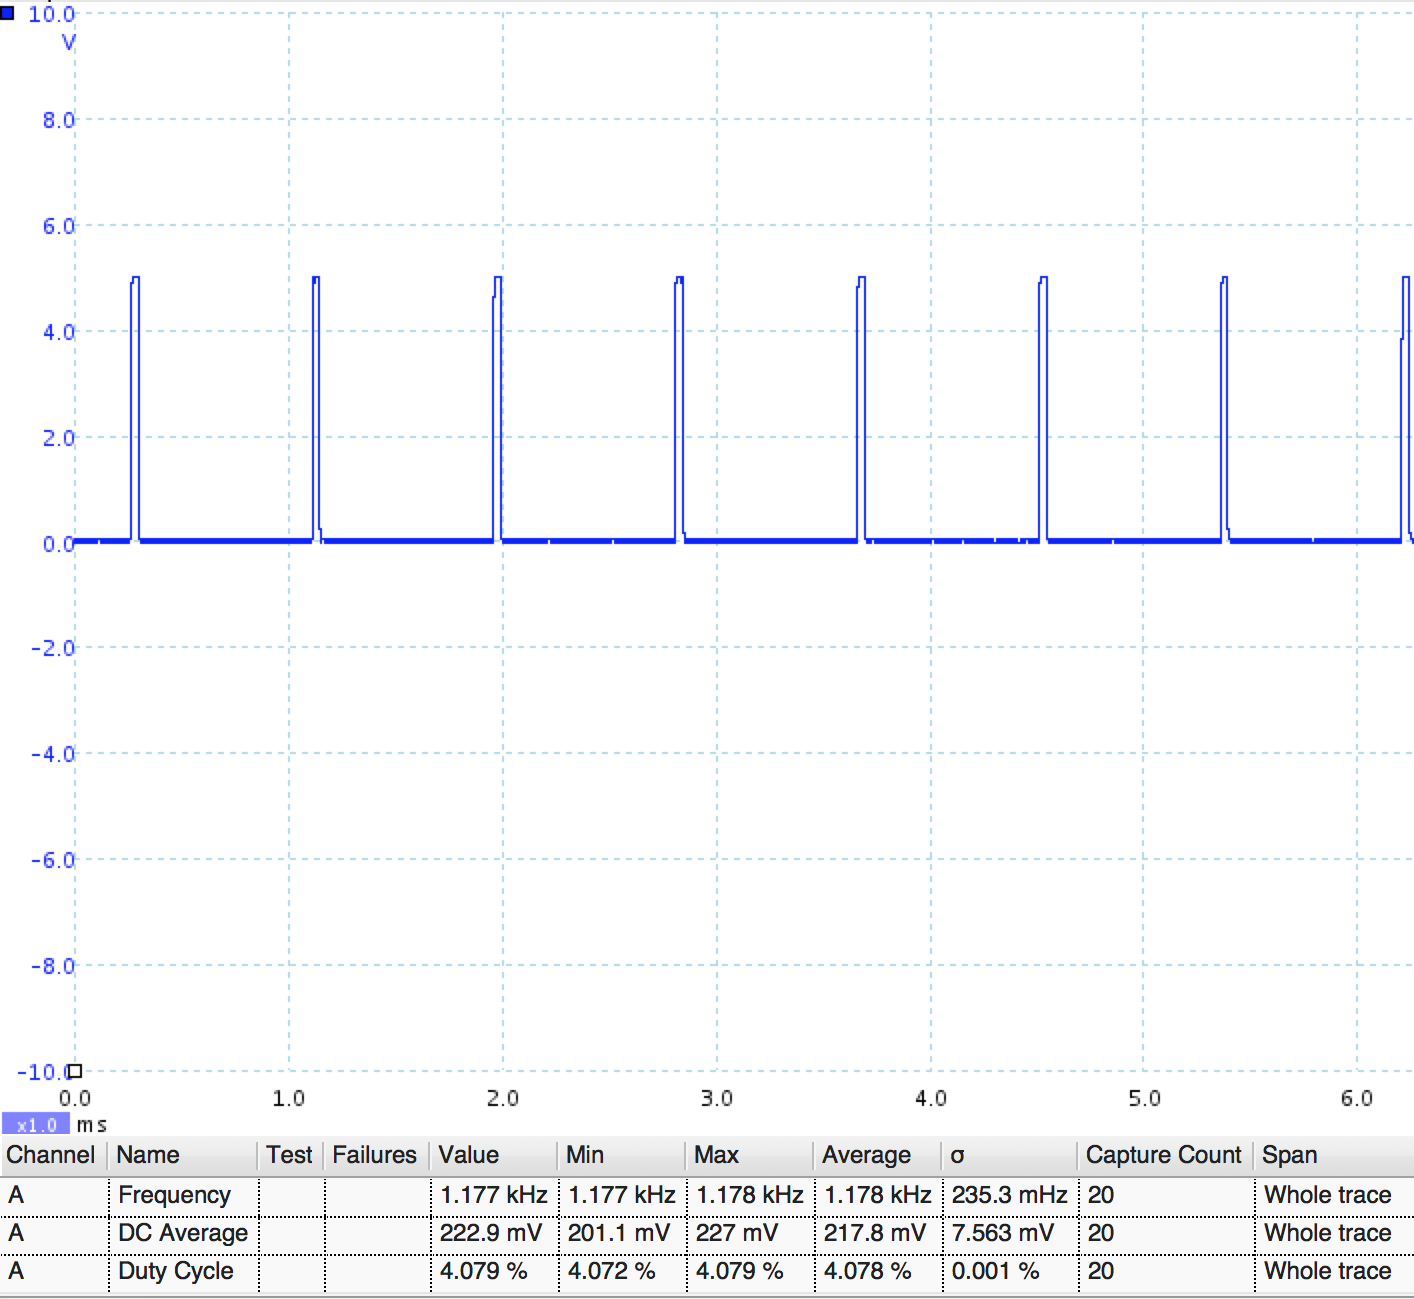
\includegraphics[width=13cm]{figures/2_4_3hastighed/555signalinv.png}
	\caption{Det inverterede signal som funktion af tiden med info-bokse i bunden}
	\label{fig:555inv}
\end{figure}

\begin{figure}[H]
	\centering
    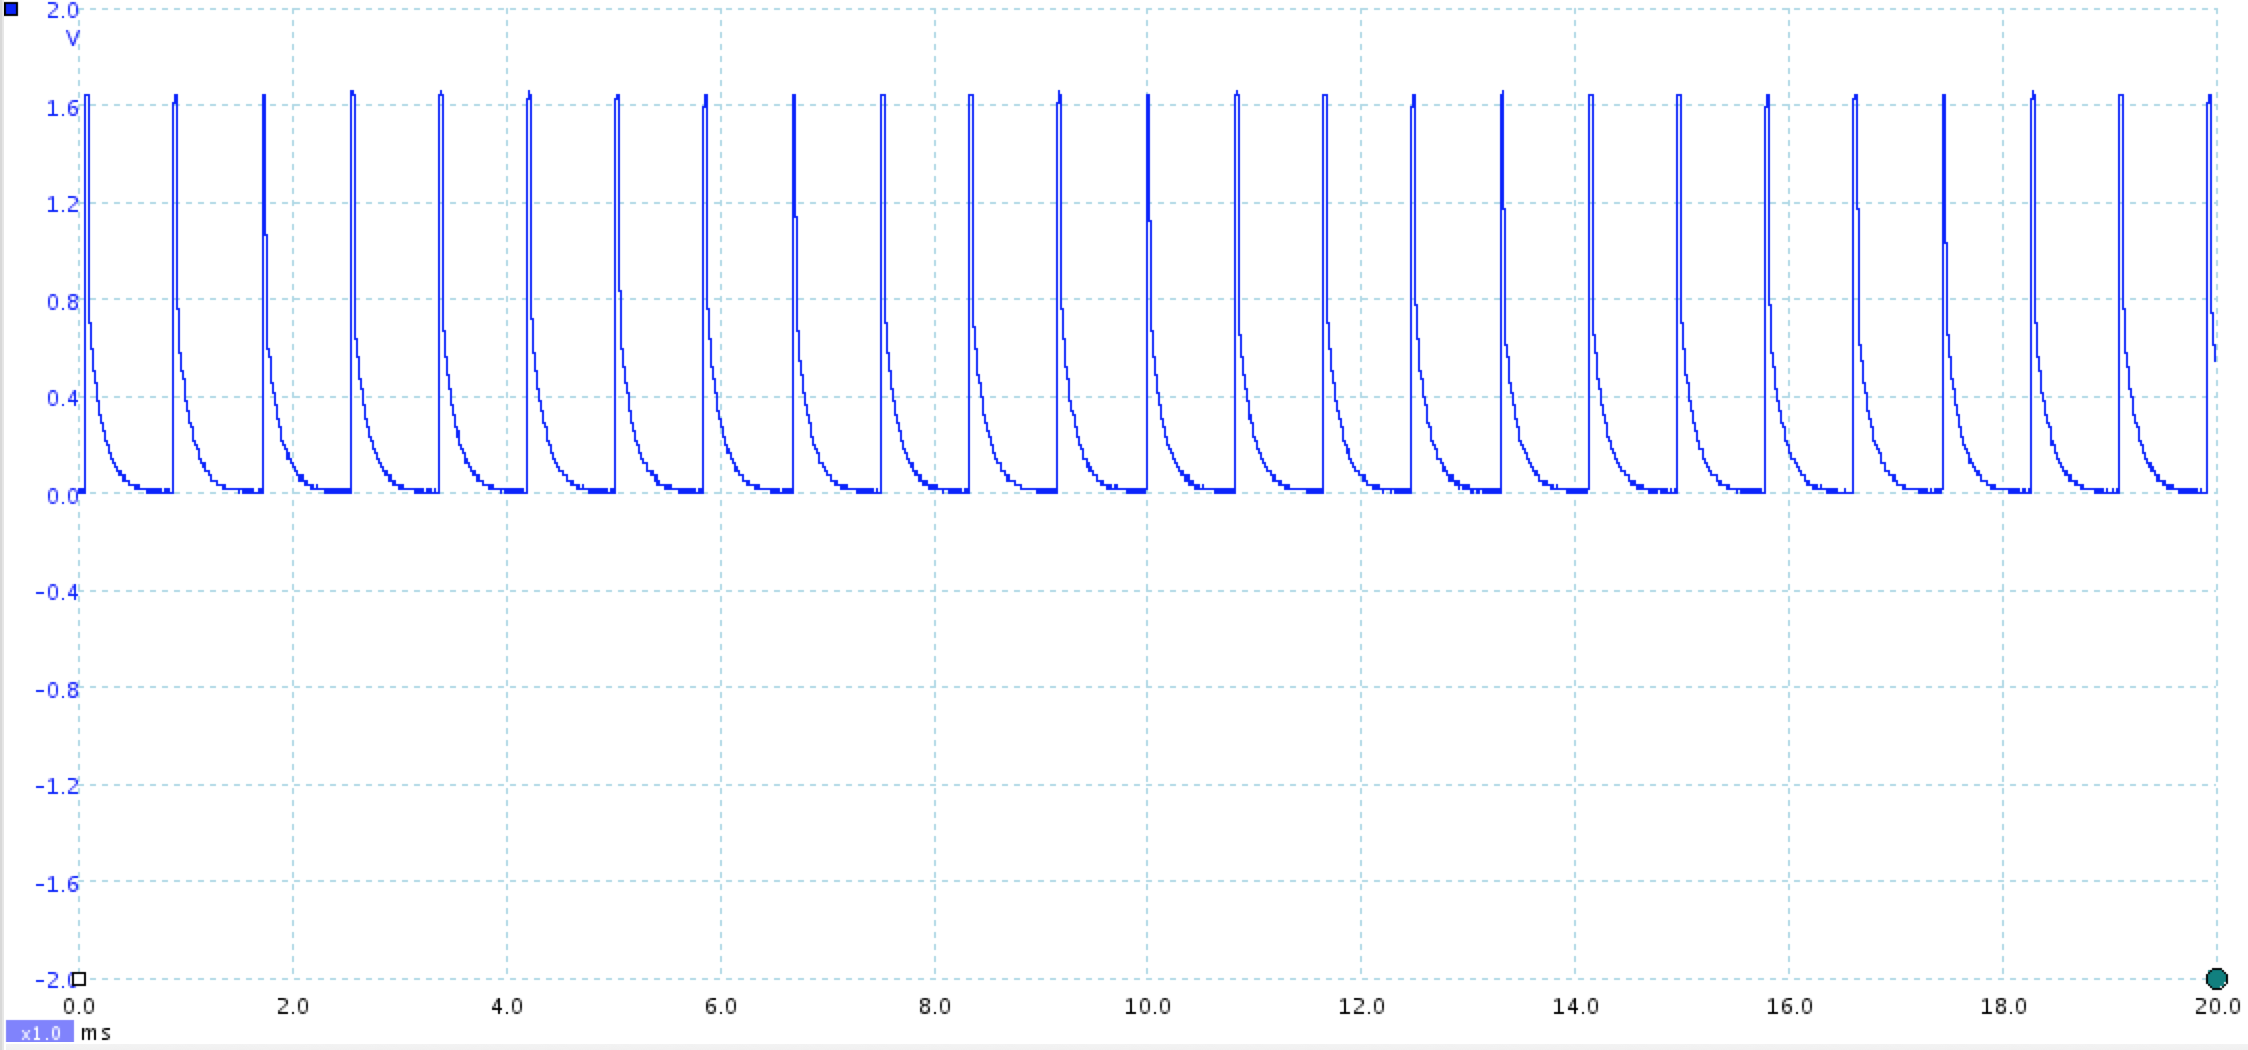
\includegraphics[width=13cm]{figures/2_4_3hastighed/555timerDiode.png}
	\caption{Spænding over dioden som funktion af tiden}
	\label{fig:diodeafsender}
\end{figure}
% 12/(10*10^(-3))
Spændingen over dioden kan ses på Figur ~\ref{fig:diodeafsender}.
Frekvensen estimeres ud fra de 12 første bølgetoppe. Heraf bemærkes at 

\[
	f_{diode} \approx \frac{12}{\SI{10d3}{s}} = \SI{1200}{Hz}
\]
Hvilket svarer fint til frekvensen af outputtet fra 555-timeren.

\subsubsection{Modtager dioden}
For modtager-delen af kredsen fremgår det på \ref{fig:IR_modtager} at frekvensen er omtrent $\SI{1.4d3}{Hz}$, og et tydelig spændingsforskel på omtrent $-\SI{5}{V}$ hvilket er et fint og tydeligt signal.
\todo{vi kunne muligvis godt have mere tekst her}
\begin{figure}[H]
	\centering
    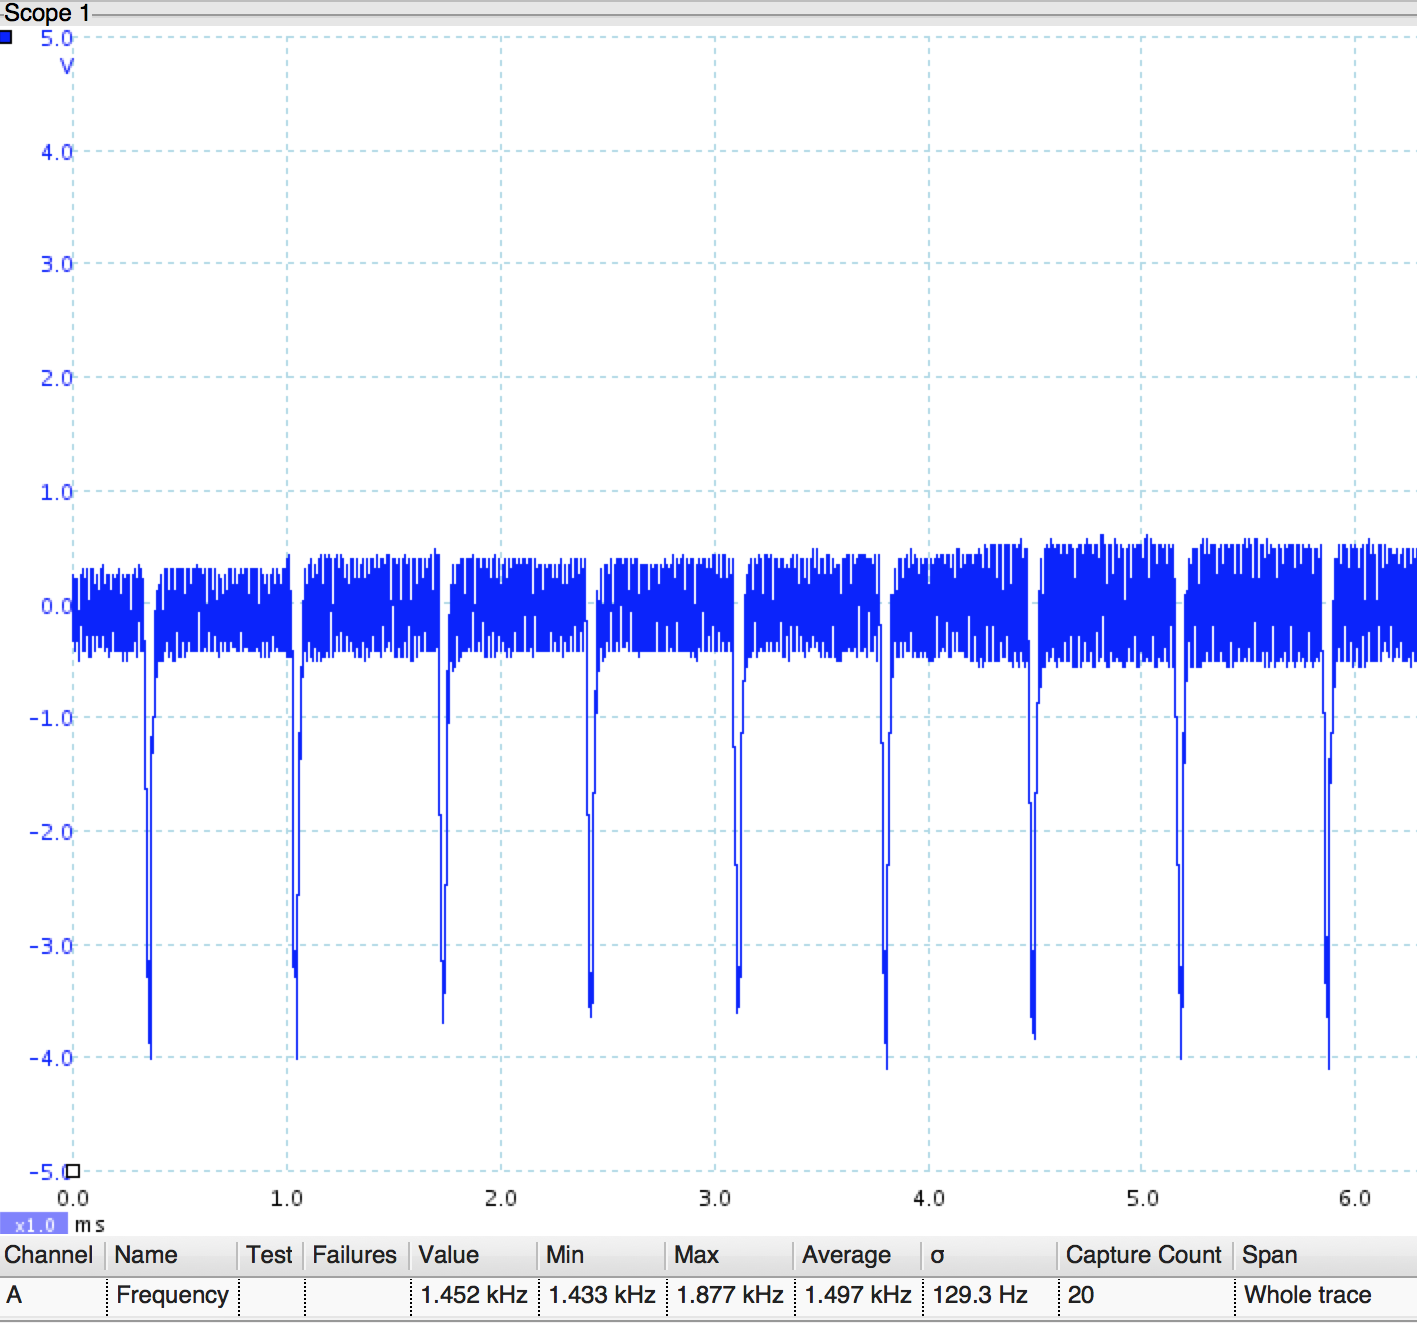
\includegraphics[width=13cm]{figures/2_4_3hastighed/IR_modtager.png}
	\caption{Spændingen som funktion af tiden af modtagerkredsens signal}
	\label{fig:IR_modtager}
\end{figure}

















